\section{Evaluation}
\label{sec:evaluation}
DCG-UPUP-Away is evaluated in two experiments.
First, a simulated turtlebot within randomly generated simulated environments is given a series of user-generated natural language commands.
Second, a physical turtlebot is given specific commands in a laboratory environment in order to demonstrate novel behaviors enabled by DCG-UPUP-Away.
Both experiments assume a perfect object recognizer that translates raw sensor data into a world model $\Upsilon$ that may be used by DCG-UPUP-Away, as well as an initial set of hand-labeled training examples for training the LLM to ground cubes, spheres, and cylinders.\\
\subsection{Experimental Setup}
\indent The simulated testing environments are randomly generated in Gazebo.
10 worlds are created, and each is populated with a random collection of objects in randomized locations.
There are 8 possible object types (including cubes, spheres, and cylinders) in 3 possible colors, for a total of 24 objects.
Each object has a 15\% chance of being added to a given map.\\
\indent After generating the 10 maps, screenshots of world with a single object highlighted are uploaded to Amazon Mechanical Turk.
For each image, users were instructed to write a command ``for approaching the highlighted object.''
These image-command pairs are then saved for evaluating whether a robot, when placed in the corresponding simulated world and given the natural language command, successfully approaches the correct object.
An example screenshot, with an annotation supplied by a user, is shown in Figure~\ref{fig:amt}.\\
\begin{figure}[h]
	\centering
    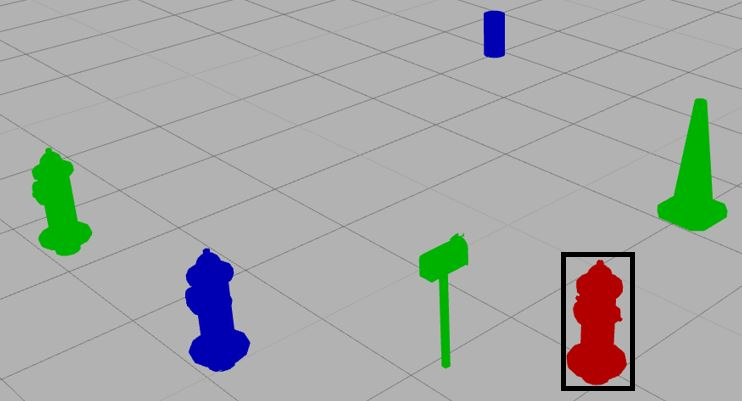
\includegraphics[width=8.5cm]{amt}
	\caption{A simulated world with a highlighted object presented on Amazon Mechanical Turk, labeled by a user as ``Move to the red fire hydrant.''}
	\label{fig:amt}
\end{figure}
The metrics we consider are the grounding accuracy (how likely DCG-UPUP-Away is to correctly ground a phrase) and the number of known symbols.

\subsection{Grounding Accuracy}
here I show the grounding accuracy (as well as how need hypothetical groundings)

I plot the grounding accuracy.
\begin{figure}[h]
\centering
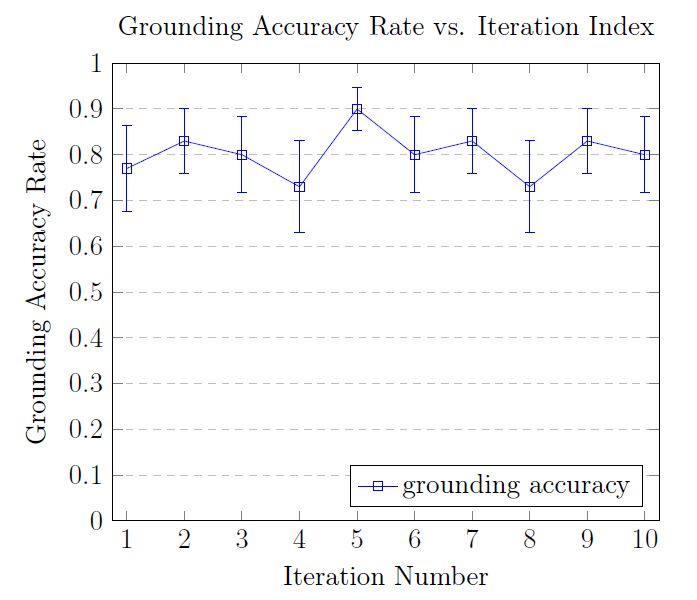
\includegraphics[width=8.5cm]{g_acc}
\caption{this is the overall grounding accuracy}
\label{fig:g_acc}
\end{figure}

Here I split up the success cases, normalized by the overall accuracy rate, for known, unknown, and learned.
\begin{figure}[h]
\centering
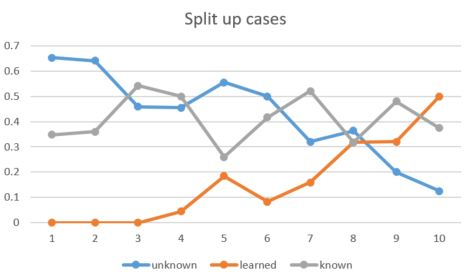
\includegraphics[width=8.5cm]{learning}
\caption{this is split up (must replot well)}
\label{fig:g_acc}
\end{figure}


\subsection{Learned Symbols}
here I show how DCG-UPUP-Away learns symbols
\begin{figure}[h]
\centering
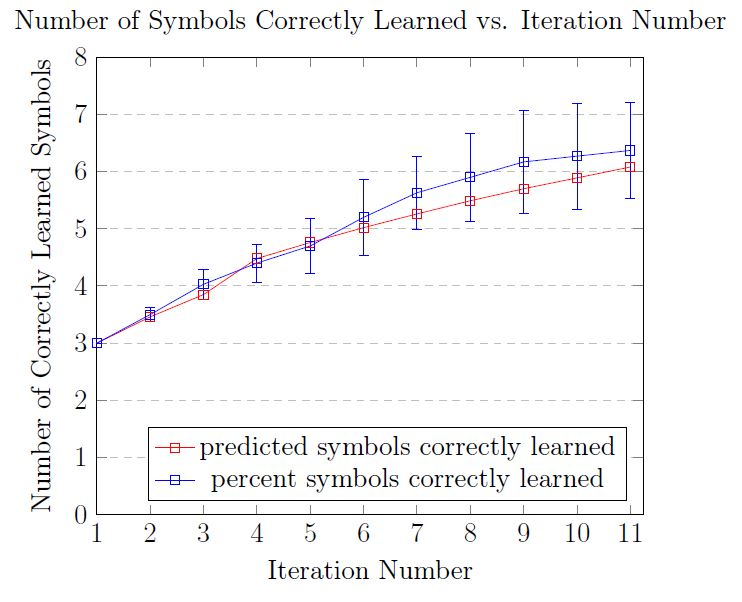
\includegraphics[width=8.5cm]{symbols_corr}
\caption{this is how we show that we learn symbols}
\label{fig:g_acc}
\end{figure}

\subsection{Hardware Demonstration}
here I show how this works on hardware.
I will say how it works in the 4 cases: known perceived (KP), known hypothesized (KH), unknown perceived (UP), and unknown hypothesized (UH).
Here is a sketch of a final figure I'd like to include:

\begin{figure}[h]
\centering
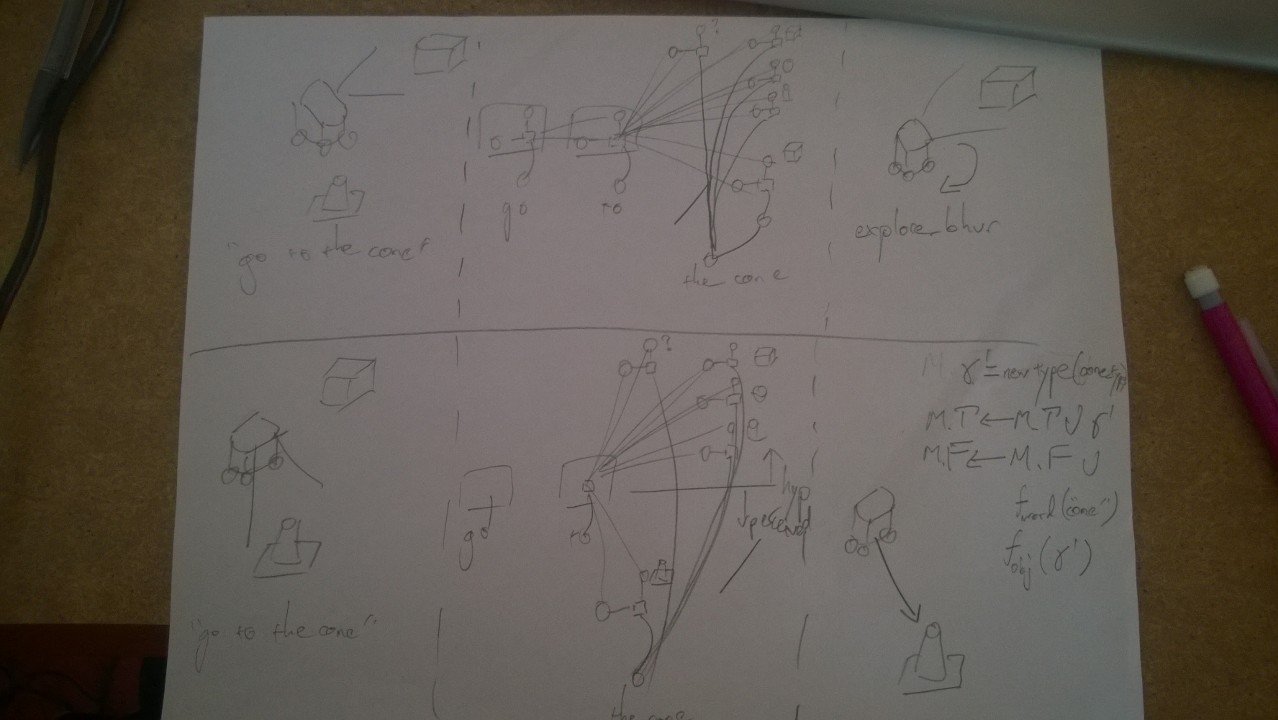
\includegraphics[width=8.5cm]{hardware_sketch}
\caption{this is a sketch of the 6 subfigures that demonstrate hypothesized groundings on hardware and in the model, and shows how it learns.}
\label{fig:g_acc}
\end{figure}

\subsection{Limitations}
here I saw what the limitations are